\section{Tricks}

Although my tutor has told me that he doesn't care about the tricks and details, 
but code still runs on these tricks and details.
I will list some detailed tricks here, 
which is of great significnce to running program properly.

\subsection{The Direaction of $\nabla W_{ij}$ and Low Pressure Problem}

As mentioned above, $\nabla W_{ij}$ has the direction as $\vec{r}_i - \vec{r}_j$.
However, as $W^\prime(q)$ is below zero, 
thus actually $\nabla W_{ij}$ has the direction as $\vec{r}_j - \vec{r}_i$:

\begin{figure}[H]
    \centering
    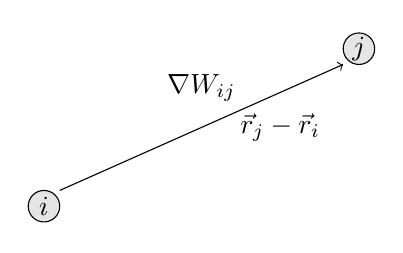
\begin{tikzpicture}
        \filldraw[fill=gray!20!white, draw=black] (0,0) circle (0.2);
        \filldraw[fill=gray!20!white, draw=black] (4,2) circle (0.2);

        \node at (0,0) {$i$};
        \node at (4,2) {$j$};

        \node at (3.0, 1) {$\vec{r}_j - \vec{r}_i$};
        % arrow without head
        \draw[->] (0.2,0.2)--(3.8,1.8);
        
        \node at (2, 1.5) {$\nabla W_{ij}$};
    \end{tikzpicture}
\end{figure}

Let's turn to the continuity equation in SPH method:
\begin{equation}
    \frac{d\rho_i}{dt} = \sum_j m_j \vec{u}_{ij} \cdot \nabla W_{ij}
\end{equation}
as long as 2 particles approach each other, 
$\vec{u}_{ij}\cdot \nabla W_{ij}$ will be positive, 
leading to an increase of $\rho_i$ and $\rho_j$.
You may see that the increase of density is symmetric to these 2 particles.

When eq.\ref{eq:Weakly Compressible Scheme} is introduced, 
a problem arises that particles captures lower density ($\rho<\rho_0\to$negative pressure) 
will get together from motion equation.
A group of particles approaching each other will cause a large increase on density 
as well as a sharp increase on pressure.
High pressure field will push these particles away from each other, 
and emit them out like a bullet.

\begin{figure}[H]
    \centering
    \subfigure[low pressure field in calculation]{
        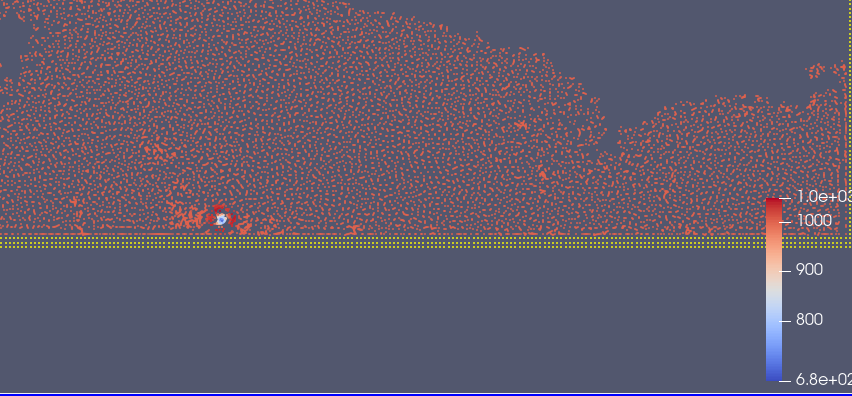
\includegraphics[width=0.4\textwidth]{images/low_pressure_field.png}
    }
    \subfigure[emit particles out like bullets]{
        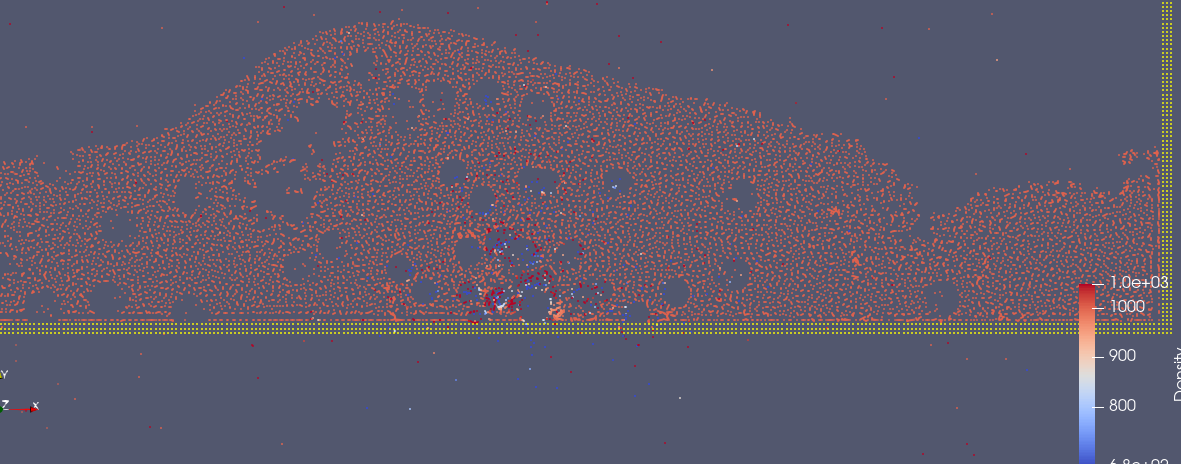
\includegraphics[width=0.48\textwidth]{images/emit_like_bullet.png}
    }
\end{figure}

It's worth noting that a ratio of smoothing length $h$ and particle's initial gap $\mathrm{d}r$ 
will influence the calculation result.
When $h/\mathrm{d}r$ is small, 
a particle is influenced by a few particles around it.
And the fluid will flow more loosely like 'ocean balls' in children's playground.
When $h/\mathrm{d}r$ is large, 
a particle is influenced by a lot of particles around it.
And the fluid will flow more tightly like 'water' in a glass.

Although for high numerical pricision, 
$h/\mathrm{d}r$ should be as large as possible, 
this may cause the low pressure problem leading to numerical instability.
In my personal practice,
I found that $h/\mathrm{d}r=3$ corresponds to reference's result, 
but will cause low pressure problem at the same time in standard case collapse onto dry bottom.

To conclude, 
we should avoid particles with low density getting together in weakly-compressible-state SPH method.
A possible way is to generate an artificial repulsive force between 2 particles 
added to pressure force part (inspired from Lenard-Jones repulsive force):
\begin{equation}
    \vec{f}_i^p = 
    -\sum_j 
    m_j 
    \left(
        \frac{p_i}{\rho_i^2} + \frac{p_j}{\rho_j^2} + R_{ij}
    \right)\nabla W_{ij}
\end{equation}
where $R_{ij}$ equals to ($\Delta p$ is the initial gap between 2 particles):
\begin{equation}
    R_{ij} = 
    0.01
    \left(
        \frac{p_i}{\rho_i^2} + \frac{p_j}{\rho_j^2}
    \right)
    \frac{W(r_{ij}, h)}{W(\Delta p, h)}
\end{equation}

\subsection{XSPH Method}

XSPH method was first proposed by Monaghan,
aiming at avoiding particles penetrating each other.
The main idea is to add a correction term to velocity when moving particles:
\begin{equation}
    \frac{\mathrm{d}\vec{r}_i}{\mathrm{d}t} = \vec{u}_i - \epsilon \sum_j m_j \frac{\vec{u}_{ij}}{\bar{\rho}_{ij}} W_{ij}
\end{equation}
where $\bar{\rho}_{ij} = \frac{1}{2}(\rho_i + \rho_j)$,
and $\epsilon$ varies from 0 to 1.
Monaghan suggested that $\epsilon$ should be set to $0.5$.

My tutor told me that XSPH method's parameter $\epsilon$ can be modified artificially.
At current stage, I have an initial idea that use a function to determine the 
disorder degree of particles.
The value of $\cos<\vec{u}_i, \vec{u}_j>$ can be used to measure the disorder degree of 2 particles.
When $\cos<\vec{u}_i, \vec{u}_j>$ is close to $1$, 
which means 2 particles are moving in the same direction, 
thus $\epsilon$ should be set to a small value.
When $\cos<\vec{u}_i, \vec{u}_j>$ is close to $-1$,
which means 2 particles are moving in the opposite direction,
thus $\epsilon$ should be set to a large value.

The XSPH method can be added to the SPH method easily and improves the stability,
but can't avoid low-pressure problem completely.

% red warning
\textcolor{red}{Warning, 2023.12.26:} I found that XSPH method in unsteady problem will lead to
unpredictable error when high-speed particles penetrate low-speed particles.

\subsection{Kernel Correction}

For particles close to boundary (like free surface boundary and wall boundary),
the kernel function will be cut off by boundary.
Thus a kernel correction should be applied to these particles.

\begin{figure}[H]
    \centering
    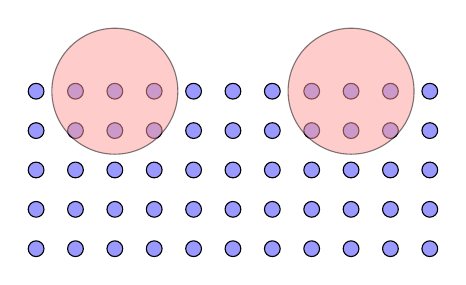
\begin{tikzpicture}
        % several particles
        % 4 row, 5 column
        \foreach \x in {0,1,2,3,4,5,6,7,8,9,10}
        \foreach \y in {0,1,2,3,4}
        \filldraw[fill=blue!40!white, draw=black] (0.5*\x,0.5*\y) circle (0.1);
        % draw a circle at the top row in the middle, alpha = 0.5
        \draw[fill=red!40!white, draw=black, opacity=0.5] (1.0,2) circle (0.8);
        % draw a circle at the top row in the middle, alpha = 0.5
        \draw[fill=red!40!white, draw=black, opacity=0.5] (4.0,2) circle (0.8);
    \end{tikzpicture}
\end{figure}
\begin{equation}
    \hat{\rho}_i = \frac{
        \sum_j m_j W_{ij}
    }{
        \sum_j \frac{m_j}{\rho_j}W_{ij}
    }
\end{equation}

For particles inside the fluid field,
kernel function which is a $\delta$-like function should gaurantee that:
\begin{equation}
    \sum_j \frac{m_j}{\rho_j} W_{ij} \approx 1
\end{equation}

This kind of kernel correction is fit for other physical quantities as well.
Any physical quantity $A$ can be corrected by:
\begin{equation}
    \hat{A}_i = \frac{
        \sum_j \frac{m_j}{\rho_j} A_j W_{ij}
    }{
        \sum_j \frac{m_j}{\rho_j} W_{ij}
    }
\end{equation}

Kernel correction is not necessary in each time step. 
A recommended time step interval is 30 time steps.
It's of great significnce to gaurantee calculation stability.

\subsection{Design of Compulsive Boundary Condition}

Compulsive boundary condition is applied by aranging a group of wall 
particles at the boundary.
As is mentioned above,
this compulsive boundary condition is designed by a singular function:
\begin{equation}
    f(q) = \frac{1}{\sqrt{q}}(1-q) \quad q=\frac{\psi}{2h}
\end{equation}

\begin{figure}[H]
    \centering
    \begin{tikzpicture}
        % plot f(q)
        \draw[->] (-0.5,0)--(1.5,0) node[right] {$q$};
        \draw[->] (0,-0.5)--(0,1.8) node[above] {$f(q)$};
        \draw[domain=0.1:1, samples=100] plot(\x, {0.5*1/sqrt(\x)*(1-\x)});
    \end{tikzpicture}
\end{figure}

This function will meet a sharp increase as $q$ approaches $0$ from $1$.
When a pair of fluid particle and wall particle is close enough at initial time,
the compulsive force will be very large and push the fluid particle away from the wall particle,
resulting in a non-physics result.
Although Monaghan proposed that $q=\psi/2\Delta p$ and papers citing his article 
proposed that $q=\psi/2h$.
No matter which one is used,
the main idea is to avoid initial gap between fluid particle and wall particle being smaller 
than the influence radius of $f(q)$.
\begin{figure}[H]
    \centering
    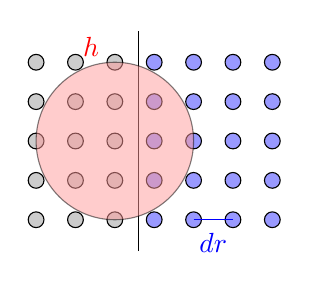
\begin{tikzpicture}
        % fluid particle
        \foreach \x in {0,1,2,3}
        \foreach \y in {0,1,2,3,4}
        \filldraw[fill=blue!40!white, draw=black] (0.5*\x,0.5*\y) circle (0.1);
        \draw[-] (-0.2,-0.4) -- (-0.2,2.4);
        % boundary particle
        \foreach \x in {-3,-2,-1}
        \foreach \y in {0,1,2,3,4}
        \filldraw[fill=gray!40!white, draw=black] (0.5*\x,0.5*\y) circle (0.1);
        
        \filldraw[fill=red!40!white, draw=black,opacity=0.5] (-0.5,0.5*2) circle (1.);

        \node[red] at (-0.8,2.2) {$h$};

        \draw[-,blue] (0.5,0) -- (1,0);
        \node[blue] at (0.75,-0.3) {$dr$};
    \end{tikzpicture}
\end{figure}

What's more, 
Monaghan said the detaild form of $f(q)$ is not important as long as 
$f(q)$ has the property of $f(0)=\infty$ and $f(1)=0$.
However, in my personal practice,
the coefficient is still important which determines the stiffness of compulsive boundary condition.
The fluid particle's splashing speed largely depend on this.

\subsection{Background Pressure}

In senior-high-school physics,
the atmospheric pressure is about $101325\mathrm{Pa}$.
This part is usually ignored in steady water field.

Here's always a problem I can't understand in SPH that:
\begin{equation}
    \phi\nabla p = \nabla (\phi p) - p\nabla \phi
\end{equation}

Apply $\nabla$'s operator with kernel interpolation method:
\begin{equation}
    \begin{aligned}
        \phi_i\nabla p_i
    &= \sum_j 
    \frac{m_j}{\rho_j} \phi_j p_j \nabla_i W_{ij}
    -\sum_j
    p_i\frac{m_j}{\rho_j} \phi_i \nabla W_{ij}\\
    \nabla p_i
    &=
    \frac{1}{\phi_i}\sum_j
    \frac{m_j}{\rho_j} \phi_j (p_j-p_i) \nabla W_{ij}
    \end{aligned}
\end{equation}
let $\phi=1$ we have:
\begin{equation}
    \nabla p_i
    =
    \sum_j
    \frac{m_j}{\rho_j} (p_j-p_i) \nabla W_{ij}
\end{equation}

This format of kernel interpolation is correct but not usually widely applied in 
SPH. Instead, the following format is widely used:
\begin{equation}
    \nabla p_i
    =\rho_i
    \sum_j m_j
    \left(
        \frac{p_i}{\rho_i^2} + \frac{p_j}{\rho_j^2}
    \right)\nabla W_{ij}
\end{equation}

When background is added into each particle's pressure,
the 2 kernel interpolation methods are quite different.
$p_j-p_i$ part neglects the background pressure, 
while $\frac{p_i}{\rho_i^2} + \frac{p_j}{\rho_j^2}$ scheme
will have an extra part $p_0\left(
    \frac{1}{\rho_i^2} + \frac{1}{\rho_j^2}
\right)$.

A possible reason is that SPH method
uses $\delta$-like function as kernel function, which actually
performs as a probability distribution like wave function in quantum mechanics.
This indicates that SPH method requires a large number of neighbour particles to
eliminate the influence of single one nearby particle.
Thus focus on 2 particles' interaction may not reflect the real physical phenomenon.
From perspective of probability,
SPH kernel interpolation method uses enough particles to approximate the real physical phenomenon,
just like Large Number Law.

With this in mind, 
a particle's front and back neighbour particles will 
balance the background pressure as to kernel interpolation on the particle itself.

Thus when background pressure is added, 
gas particles capturing with constant atmospheric pressure should be 
included into calculation, which is useless for water field simulation.

\subsection{$\delta^+$ SPH Model: A Kind of Density Filter and Stabilizer}

$\delta^+$ SPH model is adopted to avoid pressure oscillation.
For in SPH, pressure only depends on density, 
thus the stability of density field is of great significnce.

With this in mind, an additional part is added to continuity equation:
\begin{equation}
    \left(
        \frac{\partial \rho}{\partial t}
    \right)_i
    =
    \sum_j m_j \vec{u}_{ij} \cdot \nabla W_{ij}
    +
    h c_0 \delta
    \sum_j  \frac{m_j}{\rho_j} \vec{D}_{ij}\cdot \nabla W_{ij}
\end{equation}
$\vec{D}_{ij}$'s part is complicated. We first propose a concept of re-normalization matrix 
$[L]_i$ as below (tensor multiply instead of dot contraction):
\begin{equation}
    [L]_i = \left[\sum_j \frac{m_j}{\rho_j}\vec{r}_{ij}\nabla W_{ij}\right]^{-1}
\end{equation}
$[L]_i$ has the size of $d\times d$ where $d$ is the dimension of space.

The matrix is a kind of "Unit" matrix, 
where the re-normalized gradient of density $\nabla \rho_i^L$ can be calculated by:
\begin{equation}
    \nabla \rho_i^L = \sum_j \frac{m_j}{\rho_j}\rho_{ij}
    [L]_i \cdot \nabla W_{ij}
\end{equation}

Finally, $\vec{D}_{ij}$ is given by:
\begin{equation}
    \vec{D}_{ij} = 
    \left[
        2\rho_{ij} - 
        \left(
            \nabla \rho_i^L + \nabla \rho_j^L
        \right)\cdot \vec{r}_{ij}
    \right]
    \frac{\vec{r}_{ij}}{r_{ij}^2 + 0.01h^2}
\end{equation}

$\delta$ is a dimensionless parameter, 
which is usually set to $0.1$.
As described in Monaghan's paper,
$\delta^+$ SPH model is a kind of density filter and stabilizer,
which can even lead to better results than ICSPH in WCSPH method.

% warning
\textcolor{red}{Warning, 2023.12.26:} Application of $\delta^+$ SPH model 
will lead to sharp increase of calculation time.
In my personal practice, 
about 6 times much more time is needed in $\delta^+$ SPH.
Maybe a simple kernel correction is enough to stabilize the density field.